\chapter{ทฤษฎี และเทคโนโลยีที่เกี่ยวข้อง}
\label{chapter:literature-review}

\section{ทฤษฎี และงานวิจัยที่เกี่ยวข้อง}
\subsection{การคิดเชิงคำนวณ (Computational Thinking)}
การคิดเชิงคำนวณคือกระบวนการแก้ไขปัญหาโดยทำการวิเคราะห์ ตีความ และทำความเข้าใจปัญหา แบ่งย่อยปัญหาที่ซับซ้อนให้ออกมาเป็นหลาย ๆ ส่วน และทำการแก้ปัญหาแบบเป็นขั้นตอน

Jeannette M. Wing นักวิจัยด้านวิทยาการคอมพิวเตอร์ กล่าวว่า การคิดเชิงคำนวณเกี่ยวข้องกับการแก้ไขปัญหา การออกแบบระบบ และการทำความเข้าใจพฤติกรรมของมนุษย์โดยอาศัยแนวคิดพื้นฐานของวิทยาการคอมพิวเตอร์ \cite{ComputationalThinking} โดยการคิดเชิงคำนวณนั้นประกอบไปด้วย 4 แนวคิดสำคัญ ได้แก่
\begin{enumerate}
    \item การแบ่งย่อยปัญหา (Decomposition) แบ่งปัญหาที่มีความซับซ้อนออกเป็นหลาย ๆ ส่วนเพื่อให้ง่ายต่อการจัดการแก้ปัญหานั้น
    \item การเข้าใจรูปแบบ (Pattern Recognition) หารูปแบบที่เหมือนหรือคล้ายกันของแต่ละปัญหาที่เคยเกิดขึ้น
    \item ความคิดเชิงนามธรรม (Abstraction) สามารถระบุถึงปัญหาหลักหรือปัญหาที่เกี่ยวข้องได้
    \item การออกแบบขั้นตอนวิธี (Algorithm Design) ออกแบบ และพัฒนาขั้นตอนของการแก้ไขปัญหา
\end{enumerate}
โดยแต่ละแนวคิดนั้นมีความสำคัญเป็นอย่างมาก หากขาดแนวคิดใดไป การแก้ปัญหาแบบการคิดเชิงคำนวณมักจะเกิดความติดขัด และต้องกลับไปเริ่มต้นกระบวนการใหม่ตั้งแต่แนวคิดแรกอีกครั้ง

\subsection{สุขภาพตากับเด็กยุคดิจิตอล}
จากบทความของโรงพยาบาลบํารุงราษฎร์ ซึ่งมีการศึกษาเกี่ยวกับสิ่งที่ส่งผลต่อสายตาของเด็กที่มีการใช้โทรศัพท์มือถือ แทบเล็ต และหน้าจอต่าง ๆ เป็นเวลานาน
พบว่าสิ่งเหล่านี้อาจมีส่วนทำให้เกิดปัญหาสายตาในเด็กเช่น สายตาสั้น สายตาเอียง ตาแพ้แสงได้ โดยตัวอย่างปัจจัยที่ทำให้เด็กสายตาสั้นเพิ่มขึ้น ได้แก่
\begin{itemize}
    \item พันธุกรรม หากเด็กมีบุคคลในครอบครัวที่มีปัญหาสายตา เช่น สายตาสั้น สายตาเอียง ก็เป็นปัจจัยหนึ่งที่ทำให้เด็กเกิดปัญหาสายตาได้
    \item การทำกิจกรรมที่มีการใช้สายตาระยะใกล้เป็นเวลานาน ซึ่งรวมไปถึงการใช้อุปกรณ์คอมพิวเตอร์ และโทรศัพท์มือถือ
    \item ผู้ที่มีการทำกิจกรรมกลางแจ้งน้อย เนื่องจากมีการศึกษาที่กล่าวว่าวิตามินดีในแสงแดดเป็นปัจจัยที่ดีในการช่วยชะลอภาวะสายตาสั้นในเด็ก \cite{ChildrenEyesHealthCare}
\end{itemize}
และภายในบทความยังมีการกล่าวถึงอาการ Computer Vision Syndrome (CVS) หรือภาวะที่เกิดจากการใช้สายตากับคอมพิวเตอร์เป็นเวลานานโดยความรุนแรงจะเพิ่มขึ้นตามระยะเวลาในการใช้งาน
และจ้องหน้าจอคอมพิวเตอร์อย่างต่อเนื่อง ซึ่งผลกระทบที่ตามมาจากภาวะนี้เช่น ปวดเมื่อยตา ตาแห้ง แสบตา เคืองตา แพ้แสง เป็นต้น \cite{ComputerVisionSyndrome}

\subsection{แนวคิด CS Unplugged}
CS Unplugged หรือ Computer Science Unplugged คือแนวคิดการเรียนการสอนด้านคอมพิวเตอร์สำหรับเด็กอนุบาลจนถึงชั้นประถมปลายที่มุ่งเน้นการสร้างความเข้าใจพื้นฐานของวิทยาศาสตร์คอมพิวเตอร์
และตรรกศาสตร์ผ่านการทำกิจกรรมต่าง ๆ โดยไม่ใช้คอมพิวเตอร์ เช่น เกมกระดาน บัตรคำ การ์ด หรืออุปกรณ์ต่าง ๆ ที่มีอยู่รอบตัว \cite{CSUnplugged} \cite{CSUnplugged2}

CS Unplugged นั้นเริ่มมาจากกลุ่มนักวิทยาศาสตร์ด้านคอมพิวเตอร์ชาวนิวซีแลนด์ 3 คนคือ Tim Bell กับ Ian H. Witten และ Mike Fellows ที่ได้ร่วมกันเขียนหนังสือ “Computer Science Unplugged”
ซึ่งมีเนื้อหาเกี่ยวกับกิจกรรมการเรียนรู้ที่ฝึกการคิดวิเคราะห์ และแก้ปัญหาอย่างเป็นระบบโดยไม่ต้องอาศัยการใช้คอมพิวเตอร์ โดยจะเน้นไปที่การมีปฏิสัมพันธ์กับเพื่อนหรือบุคคลในชั้นเรียน สร้างความสนุกสนาน และสอดแทรกสาระไปพร้อม ๆ กัน

ปัจจุบันแนวคิด CS Unplugged ได้รับความนิยมอย่างแพร่หลายไปทั่วโลก และมีการแปลหนังสือ “Computer Science Unplugged” ไปเป็นภาษาต่าง ๆ อีกมากมาย สำหรับภาษาไทยได้รับการแปลโดยอาจารย์
และนักศึกษามหาวิทยาลัยธรรมศาสตร์ในชื่อ “ซีเอส อันปลั๊ก โปรแกรมเสริมสมรรถนะ และขยายความสามารถของเด็กระดับปฐมวัย (ฉบับแปลภาษาไทย)” สามารถดาวน์โหลดหนังสือได้ที่
https://resources.aiat.or.th/cs-unplugged/ หรือสามารถเข้าไปศึกษาเพิ่มเติมเกี่ยวกับแนวคิดนี้ได้ที่ https://csunplugged.org

\begin{figure}[ht]
    \centering
    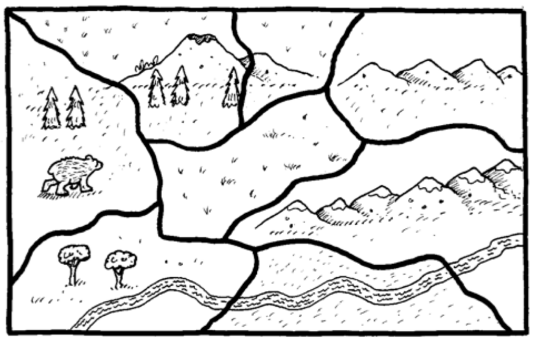
\includegraphics[width=110mm,scale=0.6]{CS-Unplugged.png}
    \caption{ตัวอย่างกิจกรรม CS Unplugged}
    \label{fig:CS-Unplugged}
\end{figure}

\section{เทคโนโลยีที่เกี่ยวข้อง}
\subsection{QR Code (รหัสคิวอาร์) \cite{VarietyOfQRCode}}
QR code มาจากคำว่า Quick Response Code โดย QR code คือบาร์โค้ดประเภท Matrix (หรือบาร์โค้ด 2 มิติ) มีลักษณะเป็นสี่เหลี่ยม ภายในประกอบไปด้วยโมดูลสีดำบนพื้นหลังสีขาว ใช้สำหรับเก็บข้อมูลประเภทข้อความซึ่งประกอบไปด้วยตัวอักษร และตัวเลข โดยในปัจจุบันมีการนำไปประยุกต์ใช้เก็บข้อมูลที่หลากหลาย เช่น ที่อยู่เว็บไซต์ (URL) ข้อความ หรือหมายเลขโทรศัพท์ 

QR code ถูกคิดค้นขึ้นที่ประเทศญี่ปุ่น โดยบริษัทเดนโซ-เวฟ (Denso-Wave) เมื่อปี พ.ศ 2537 มีความแตกต่างจาก Barcode หนึ่งมิติธรรมดาทั่วไปคือมันสามารถเก็บข้อมูลได้ 2 ทิศทาง โดยสามารถเก็บข้อมูลได้ทั้งในรูปแบบแนวตั้งหรือในรูปแบบแนวนอนซึ่งข้อแตกต่างนี้ทำให้ QR code สามารถเก็บข้อมูลได้มากกว่า Barcode หนึ่งมิติถึง 200 เท่า หรือหมายความว่ามันสามารถบรรจุข้อมูลได้มากถึง 4,000 ตัวอักษร และ 7,000 ตัวเลข

โดยการอ่าน QR code นั้นสามารถทำได้ง่าย ๆ โดยการใช้อุปกรณ์ที่มีกล้อง เช่น โทรศัพท์มือถือหรือแท็บเลตที่ได้ทำการติดตั้งโปรแกรมถอดรหัสเอาไว้แสกนไปที่ QR code จากนั้นข้อมูลที่ถูกเข้ารหัสไว้ก็จะแสดงออกมา และในปัจจุบันมี QR code เกิดขึ้นมากมายหลายประเภทจากหลายบริษัทผู้ผลิต ตัวอย่างเช่น
\begin{enumerate}[listparindent=1.25em]
    \item QR Code Model 1 และ QR Code Model 2

    เป็นรูปแบบของ QR Code ที่สามารถเห็นได้ทั่วไป และมีการใช้อย่างแพร่หลายมากที่สุดในขณะนี้ หลักการทำงานของ QR Code ชนิดนี้คือจะมีการใช้ตำแหน่งในการตรวจสอบรูปแบบ (Position detection pattern) 3 ตำแหน่งคือ ซ้ายบน ขวาบน ซ้ายล่างโดย Model 1 เป็น QR Code ตัวต้นแบบ ซึ่งขนาดที่ใหญ่ที่สุดของ Model 1 คือ เวอร์ชั่น 14 (73 x 73 โมดูล) ที่สามารถเก็บข้อมูลชนิดตัวเลขได้สูงสุดถึง 1,167 ตัว 

    Model 2 ได้รับการพัฒนามาจาก Model 1 เพื่อให้ประสิทธิภาพการอ่านดียิ่งขึ้น โดย Model 2 จะอ้างถึงรูปแบบการจัดตำแหน่งที่ฝังอยู่ ทำให้สามารถอ่านได้แม้ตัว QR Code จะผิดเพี้ยนไปจากเดิมก็ตาม โดยขนาดที่ใหญ่ที่สุดของ Model 2 คือ เวอร์ชั่น 40 (177 x 177 โมดูล) ที่สามารถเก็บข้อมูลชนิดตัวเลขได้สูงสุดถึง 7,089 ตัว ซึ่งในปัจจุบัน Model 2 คือรูปแบบที่นิยมมากที่สุด
    \begin{figure}[ht]
        \centering
        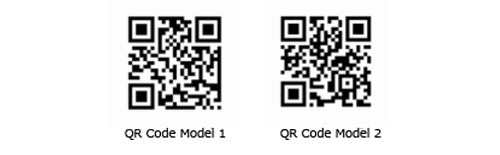
\includegraphics[width=110mm,scale=0.6]{qrcode_model1and2.png}
        \caption{QR Code Model 1 และ QR Code Model 2}
        \label{fig:qrcode_model1and2}
    \end{figure}

    \item Micro QR Code

    Micro QR Code คือ QR Code ที่มีขนาดเล็กกว่า QR Code ปกติ มีการใช้ตำแหน่งในการตรวจสอบรูปแบบ (Position detection pattern) เพียง 1 ตำแหน่ง เพื่อเป็นการลดขนาดของ QR Code โดย Micro QR Code มี 4 เวอร์ชั่น ขนาดเล็กที่สุดคือ 11 x 11 โมดูล และขนาดใหญ่สุดคือ 17 x 17 โมดูลที่สามารถเก็บข้อมูลตัวเลขได้ถึง 35 ตัว นิยมใช้บนบรรจุภัณฑ์ของผลิตภัณฑ์
    \begin{figure}[ht]
        \centering
        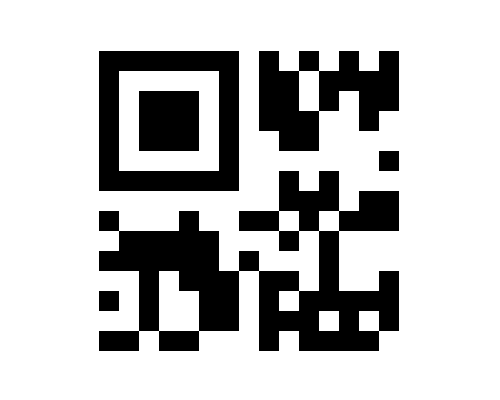
\includegraphics[width=40mm,scale=0.6]{microqr.png}
        \caption{Micro QR Code}
        \label{fig:microqr}
    \end{figure}

    \item iQR Code

    QR Code รูปแบบนี้สามารถผลิตได้ 2 รูปทรงคือแบบสี่เหลี่ยมจัตุรัส และแบบสี่เหลี่ยมผืนผ้า ขนาดใหญ่ที่สุดคือ เวอร์ชั่น 61 (422x422 โมดูล) ซึ่งสามารถเก็บข้อมูลตัวเลขได้ประมาณ 40,000 ตัว โดยมีการออกแบบมาเพื่อให้อ่านง่ายขึ้น และนำไปใช้ในพื้นที่จำกัดได้สะดวกมากยิ่งขึ้น นิยมนำไปใช้บนป้ายกำกับสินค้า
    \begin{figure}[ht]
        \centering
        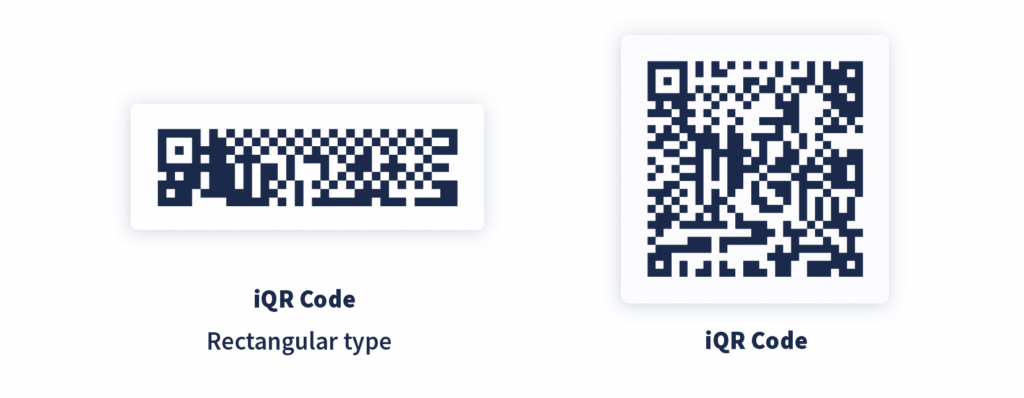
\includegraphics[width=110mm,scale=0.6]{iqrcode.png}
        \caption{iQR Code}
        \label{fig:iqrcode}
    \end{figure}

    \item SQRC Code

    SQRC Code เป็นรูปแบบของ QR Code ที่มีข้อจำกัดในการอ่านข้อมูล กล่าวคือการอ่านข้อมูลจำเป็นต้องใช้กระบวนการที่ซับซ้อนเช่นการเข้ารหัสข้อมูล และการถอดรหัสข้อมูลหลังจากทำการอ่านข้อมูลโดยอุปกรณ์ต่าง ๆ SQRC Code ได้รับการพัฒนาโดยบริษัท Denso-Wave เพื่อให้ง่ายต่อการเข้ารหัส และใช้ข้อมูลที่ไม่เปิดเผยต่อสาธารณะรวมถึงข้อมูลส่วนบุคคล และข้อมูลภายในองค์กร โดยมีรูปลักษณ์ที่เหมือนกับ QR Code ธรรมดาทุกอย่าง แต่สำหรับการอ่านจำเป็นที่จะต้องใช้เครื่องมือเฉพาะ \cite{SQRC}
    \begin{figure}[ht]
        \centering
        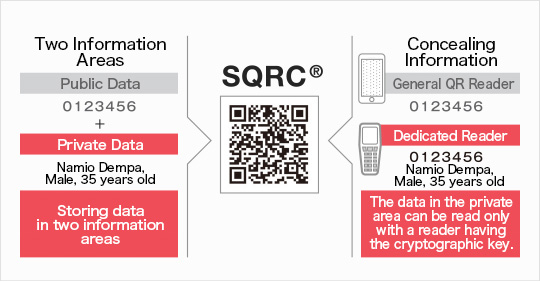
\includegraphics[width=100mm,scale=0.6]{sqrc.jpg}
        \caption{SQRC Code}
        \label{fig:sqrc}
    \end{figure}

    \pagebreak
    \item Frame QR
    
    Frame QR คือ QR Code ที่มีพื้นที่ว่างตรงกลาง (canvas area) ซึ่งสามารถนำรูปหรือตัวอักษรมาใส่ได้ และไม่มีผลต่อการอ่านข้อมูลของ QR Code นิยมนำไปใช้ในการนำเสนอสินค้าหรืออื่น ๆ ได้หลายวัตถุประสงค์
    \begin{figure}[ht]
        \centering
        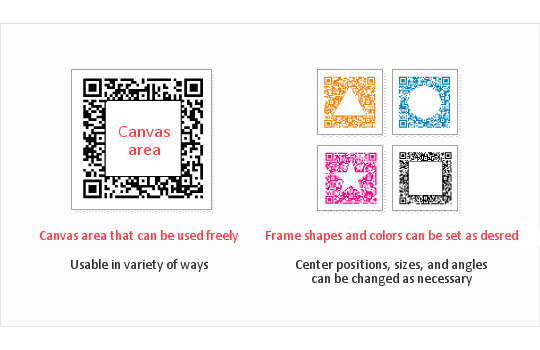
\includegraphics[width=90mm,scale=0.6]{frameqr.jpg}
        \caption{Frame QR}
        \label{fig:frameqr}
    \end{figure}

    \item HCC2D
    
    เป็นรูปแบบของ QR Code ที่ยังอยู่ในขั้นพัฒนาตัวต้นแบบ โดย QR Code ชนิดนี้จะมีการใช้สี CMYK เพื่อเพิ่มปริมาณการเก็บข้อมูล
    \begin{figure}[ht]
        \centering
        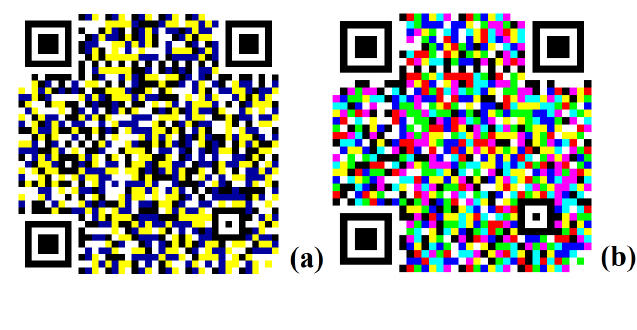
\includegraphics[width=60mm,scale=0.6]{hcc2d.png}
        \caption{HCC2D}
        \label{fig:hcc2d}
    \end{figure}

    \item LogoQ
    
    QR Code แบบใหม่ที่นำเอาโลโก้มารวมกับ QR Code ธรรมดา และนำไปสร้างใหม่ด้วย LogoQ algorithm ซึ่งมีผลลัพท์ที่ได้ตามตัวอย่างในรูปที่ \ref{fig:logoq}
    \begin{figure}[ht]
        \centering
        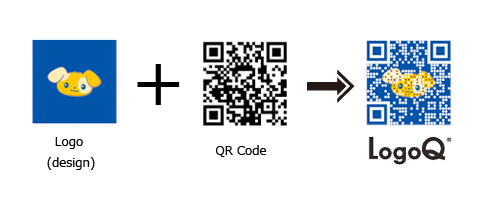
\includegraphics[width=100mm,scale=0.6]{logoq.png}
        \caption{LogoQ}
        \label{fig:logoq}
    \end{figure}

\end{enumerate}

\subsection{โมดูล ESP32 CAM}
โมดูลพิเศษซึ่งมาพร้อมกับกล้อง OV2640 ความละเอียด 2 ล้านพิกเซล และ microSD card ในตัว ใช้ชิพ ESP32 ในการเชื่อมต่อกับสัญญาณ Wi-Fi หรือ Bluetooth ที่คลื่นความถี่ 2.4 GHz
ออกแบบด้วยเทคโนโลยี TSMC พลังงานต่ำพิเศษ 40 นาโนเมตร โดย ESP32 CAM นั้น สามารถเป็นได้ทั้งตัวรับสัญญาณ และตัวปล่อยสัญญาณได้ในขณะเดียวกัน แต่ข้อเสียของมันคือไม่มีช่อง micro USB
ไว้สำหรับการอัพโหลด ทำให้ต้องอาศัย USB to TTL ร่วมด้วย \cite{ESP32CAM}
\begin{figure}[ht]
    \centering
    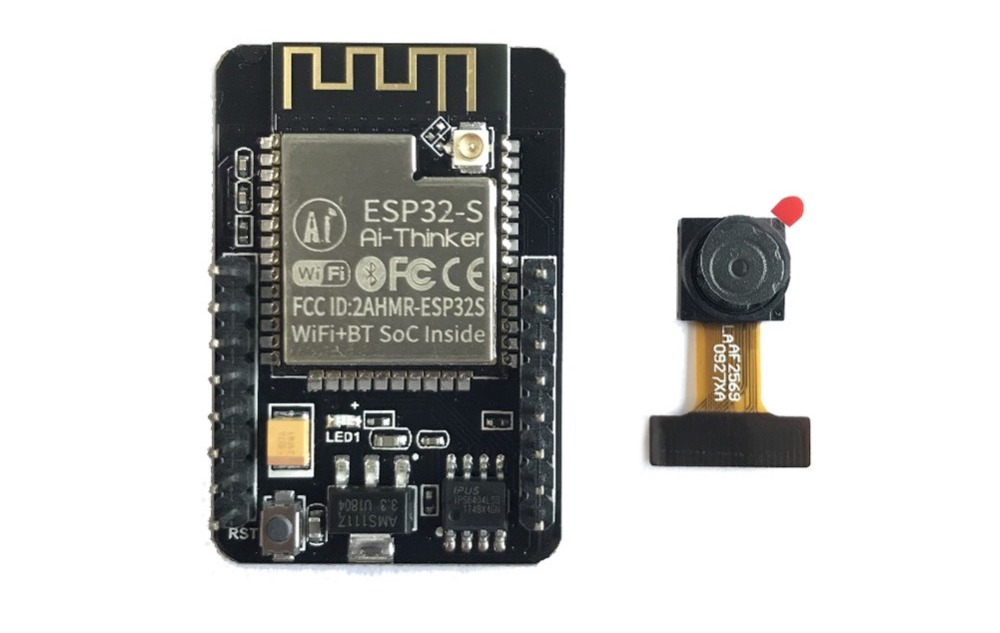
\includegraphics[width=70mm,scale=0.6]{esp32-cam.jpg}
    \caption{ESP32 CAM}
    \label{fig:esp32-cam}
\end{figure}

\subsection{L298N (Motor Driver)}

\subsection{Gear Motor}

\subsection{MicroPython}